
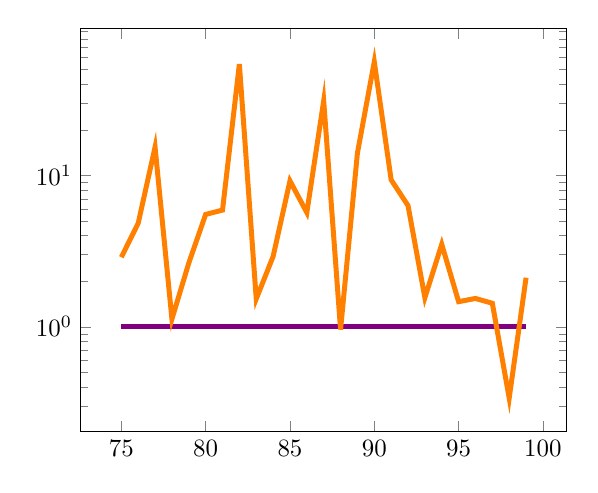
\begin{tikzpicture}[scale=0.9]
\begin{semilogyaxis}
\addplot[color=violet,line width=2pt,mark options={solid}] coordinates {(75,1.0)(76,1.0)(77,1.0)(78,1.0)(79,1.0)(80,1.0)(81,1.0)(82,1.0)(83,1.0)(84,1.0)(85,1.0)(86,1.0)(87,1.0)(88,1.0)(89,1.0)(90,1.0)(91,1.0)(92,1.0)(93,1.0)(94,1.0)(95,1.0)(96,1.0)(97,1.0)(98,1.0)(99,1.0)};
\addplot[color=orange,line width=2pt,mark options={solid}] coordinates {(75,2.883055748982736)(76,4.833448114614101)(77,15.399130233671162)(78,1.1252312217603446)(79,2.640217442645434)(80,5.528970787832903)(81,5.905456893540757)(82,54.405337554029146)(83,1.5295408651534526)(84,2.9153456395221333)(85,9.207090211348005)(86,5.687187131100625)(87,31.13257689046436)(88,0.9594627286039255)(89,14.05691234293853)(90,56.373279489941986)(91,9.35865702029314)(92,6.324456619043344)(93,1.5580073589632082)(94,3.509399111600134)(95,1.4662637163818437)(96,1.5399809784017349)(97,1.4311620808684813)(98,0.3384805957120162)(99,2.1118394007792896)};

\end{semilogyaxis}
\end{tikzpicture}
